% Sección nueva · Prototipo (componente D, 25 %). Tablero: Benja. Prueba de uso: quien la aplicó.
% Requiere en el preámbulo: graphicx, booktabs, xcolor, hyperref. Lo marcado con \pend{...} sale en rojo.
\providecommand{\pend}[1]{\textcolor{red}{#1}}

\section{Prototipo}
\label{sec:prototipo}

El prototipo es un tablero de Databricks (AI/BI) que responde la pregunta en una pantalla. Lee directo del oro de la cadena y se vuelve a publicar cada vez que la cadena corre: no tiene datos pegados a mano.\footnote{\url{https://dbc-c40c64f6-aa40.cloud.databricks.com/dashboardsv3/01f1df8721bb10a6b14af51e24530fc6/published?o=7474648132034809}. El ayudante y el profesor tienen acceso al workspace.}

\paragraph{Para quién y cada cuánto.} Para la gerencia comercial y operaciones, una vez al mes, después del cierre: en esa reunión se fija y se revisa la meta de participación de gran reserva por mercado (sección~\ref{sec:negocio}). Reemplaza la planilla que comercial arma hoy descargando el ERP a Excel (V).

\paragraph{Una pregunta en una pantalla.} La primera página sigue la anatomía de la clase~7 (figura~\ref{fig:tablero}). El título es la pregunta; debajo, el período y los filtros (moneda y fecha del dólar, correcciones, litros por caja y mercado), cada uno siempre con un valor, para que una cifra nunca mezcle escenarios. Arriba a la izquierda va la \textbf{cifra clave} con su comparación: el precio por litro subió 11,2\,\% (de 4,574 a 5,085 USD/L), la mezcla explica el 108\,\% del alza y la gran reserva pasó de 22,7\,\% a 32,5\,\% de los litros. Al lado, el \textbf{valor para decidir}: un punto de gran reserva en vez de varietal vale CLP 353 millones de margen bruto al año (338 con el dólar de la cobranza). Debajo, el \textbf{gráfico que explica la cifra}: lo que aportan mezcla, precio y cruzado junto al alza total, y la participación y el precio por litro de cada tier. Al final, el \textbf{corte por mercado} en tabla y el \textbf{pie}: última actualización, pruebas en verde, origen y fecha del dólar, período y dueño del dato.

\begin{figure}[!htbp]
  \centering
  \IfFileExists{figuras/tablero.png}%
    {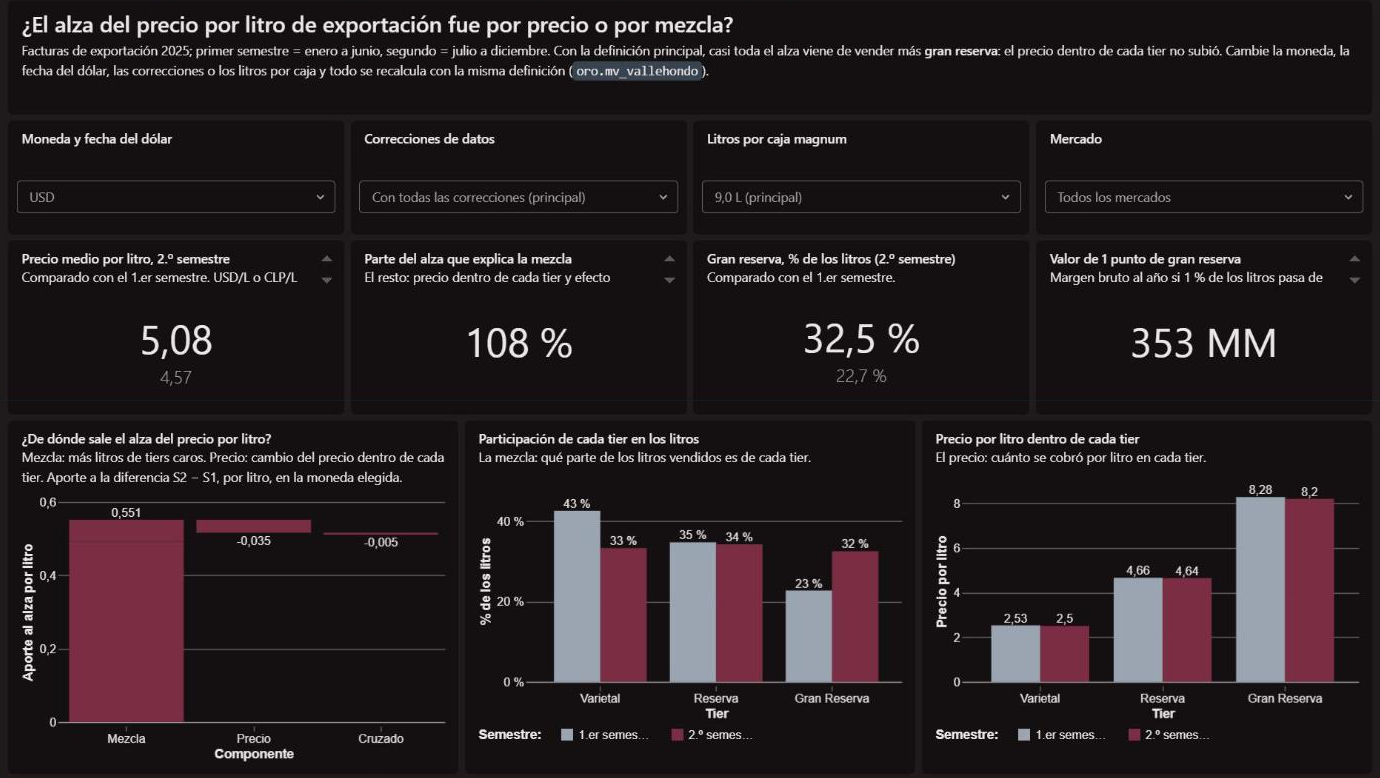
\includegraphics[width=0.66\textwidth]{tablero.png}}%
    {\fbox{\parbox[c][3.5cm][c]{0.9\textwidth}{\centering\pend{Captura de la parte superior de la página «Respuesta» (filtros, cifras clave y gráficos), subida como figuras/tablero.png}}}}
  \caption{Página «Respuesta» del tablero, con la definición principal. Fuente: tablero AI/BI de Databricks sobre el oro de la cadena.}
  \label{fig:tablero}
\end{figure}

\paragraph{Recomendación o hipótesis, con la regla escrita.} Un mercado es \emph{recomendación} si repite el patrón del total con datos suficientes: su precio por litro sube, la mezcla explica al menos el 80\,\% del alza, la gran reserva gana al menos 5 puntos, al menos el 80\,\% de sus litros tiene costo real y tiene al menos 300 líneas; si falla una condición es \emph{hipótesis}, y el tablero dice cuál. Con la definición principal los 10 mercados son recomendación, con la mezcla entre el 97\,\% y el 104\,\% del alza (M). Brasil, el único del hemisferio sur, también, con la gran reserva de 22,7\,\% a 31,5\,\%: el cambio no parece efecto de la temporada navideña del norte (I). Sin las correcciones, México pasa a hipótesis: la mezcla explicaría solo el 49\,\% de su alza.

\paragraph{La segunda página es la de la definición.} Abre con la decisión que más mueve el número: una tabla pone lado a lado el precio por litro, el alza y la parte de la mezcla en USD y con cada fecha del dólar. Debajo están el precio por tier y la gran reserva mes a mes, leídos de la definición única, las fórmulas y las 15 pruebas de la última corrida. El tablero solo filtra: con la definición principal, sus cifras son las de \texttt{cifras.md} y las de este informe.

\paragraph{Prueba de uso.} La hicieron por separado y sin ayuda Italo Suazo e Ignacio Quinteros, ingenieros que usan Power BI y son ajenos al grupo y al curso, con tres preguntas: (1)~cuánto subió el precio por litro y qué parte es mezcla; (2)~cuánto sube en pesos con el dólar de la cobranza; (3)~cuánto vale un punto de gran reserva y si Brasil es recomendación o hipótesis. Trabajaron sobre una captura de la página «Respuesta», así que no podían cambiar filtros ni bajar a la tabla de mercados. El detalle, con lo que le costó a cada uno, está en el anexo~E.

\begin{center}\footnotesize
\renewcommand{\arraystretch}{1.05}
\begin{tabular}{@{}l c c >{\raggedright\arraybackslash}p{4.4cm} >{\raggedright\arraybackslash}p{5.2cm}@{}}
\toprule
\textbf{Persona} & \textbf{Preg.} & \textbf{Tiempo} & \textbf{¿Respondió?} & \textbf{Qué cambiamos} \\
\midrule
Italo Suazo & 1 & 3 min & Sí; calculó el 11,2\,\% a mano & Cifra nueva con el alza en porcentaje \\
 & 2 & 2 min & No: dijo que con la pantalla no se podía saber & Tabla de monedas y fechas del dólar en la página 2 \\
 & 3 & 4 min & En parte: 353 MM, leídos como USD; no vio Brasil & «MM CLP» en el título del valor \\
\midrule
Ignacio Quinteros & 1 & 2 min & Sí: 11\,\% y 108\,\% & Barra del alza total en vez de la cascada \\
 & 2 & 1 min & No: había que cambiar el filtro & La misma tabla de la página 2 \\
 & 3 & 3 min & En parte: 353 MM («supongo CLP»); no vio Brasil & Textos y leyendas sin cortes \\
\bottomrule
\end{tabular}
\end{center}

\noindent La pregunta 2 tampoco se respondía con el tablero vivo sin cambiar un filtro y calcular a mano; ahora se lee en la tabla de la página 2: con el dólar de la cobranza el precio por litro en pesos sube 6,3\,\%, contra 10,1\,\% con el de la factura.

\paragraph{Lista de verificación de la clase 7.} (1) \emph{Qué pregunta responde}: si el alza del precio por litro fue por precio o por mezcla, y cuánto vale mover la mezcla. (2) \emph{Para quién y cada cuánto}: gerencia comercial y operaciones, una vez al mes. (3) \emph{Dónde está la cifra clave}: arriba a la izquierda, con su comparación contra el semestre anterior. (4) \emph{Si cada gráfico calza con su pregunta}: el del alza separa mezcla de precio, las barras por tier muestran qué tier se movió y la tabla dice en qué mercados se repite. (5) \emph{Ejes truncados y totales}: ningún eje está truncado; el gráfico del alza parte de cero y muestra el total que suman mezcla, precio y cruzado. (6) \emph{Quién certificó las definiciones del pie}: la cadena, con 15 de 15 pruebas en verde, la fuente y la fecha del dólar; el dueño del dato es el Departamento Comercial.
